\section{One dimensional solution using freeform solution}
Optical cloaking contact fingers had 
\section{blending of the two one dimensional solutions}

\section{Simulation rectangular unit cell}

\subsection{optimised for normal incidence}
\begin{figure}[h]
\centering
\begin{subfigure}{\textwidth}
\centering
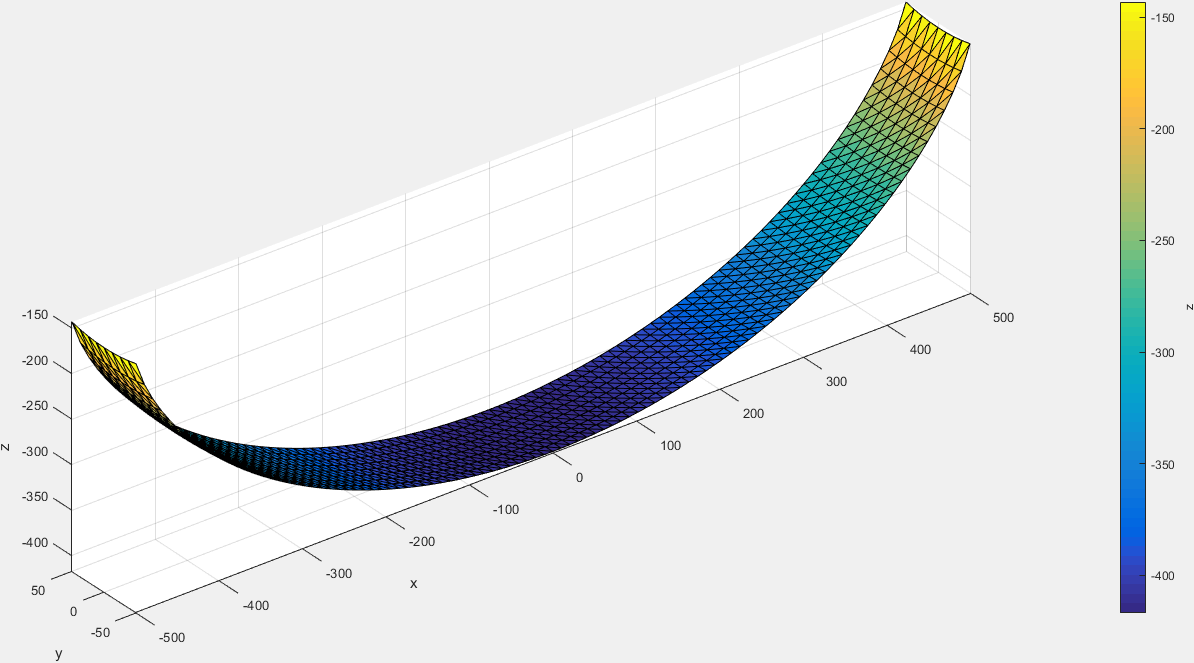
\includegraphics[width=\textwidth]{contsurf_rectangular_normal_incident_surface}
\caption{the solar cell is located at z=0 and the light is travelling in positive z direction\label{contsurf_rectangular_normal_incident_surface}}
\end{subfigure}
\begin{subfigure}{\textwidth}
\centering
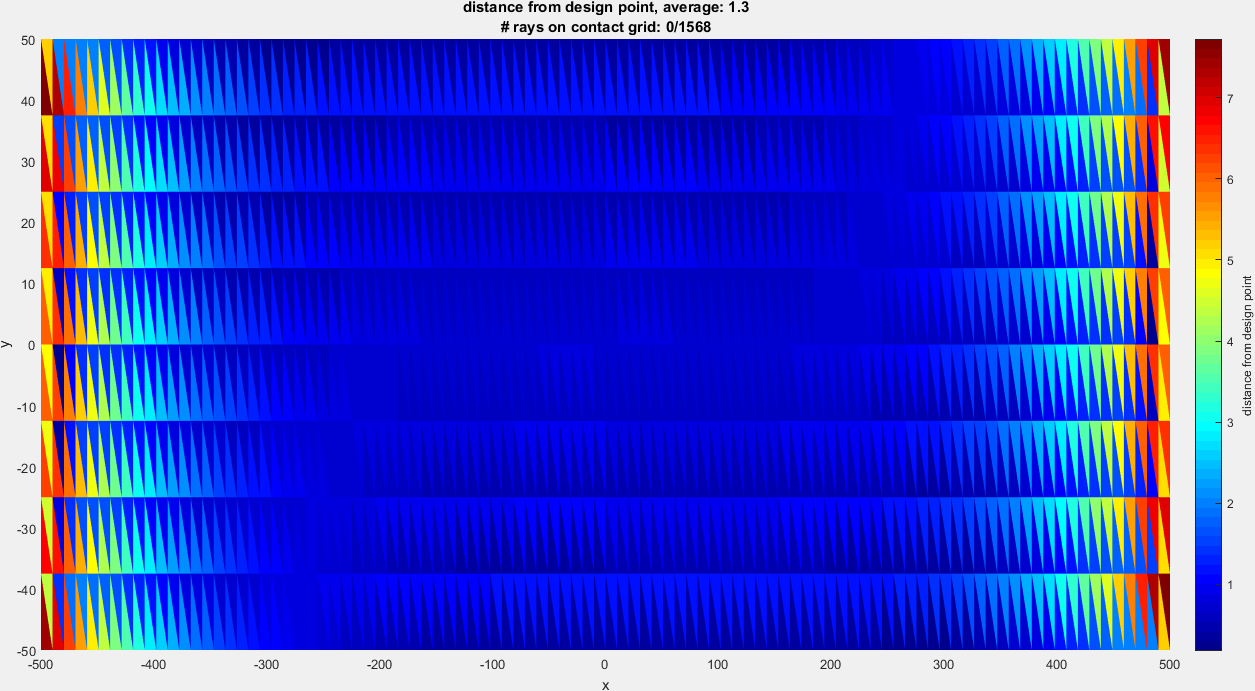
\includegraphics[width=\textwidth]{contsurf_rectangular_normal_incident_average_distance.png}
\caption{shows the average distance to the designpoint \label{contsurf_rectangular_normal_incident_average_distance}}
\end{subfigure}
\begin{subfigure}{\textwidth}
\centering
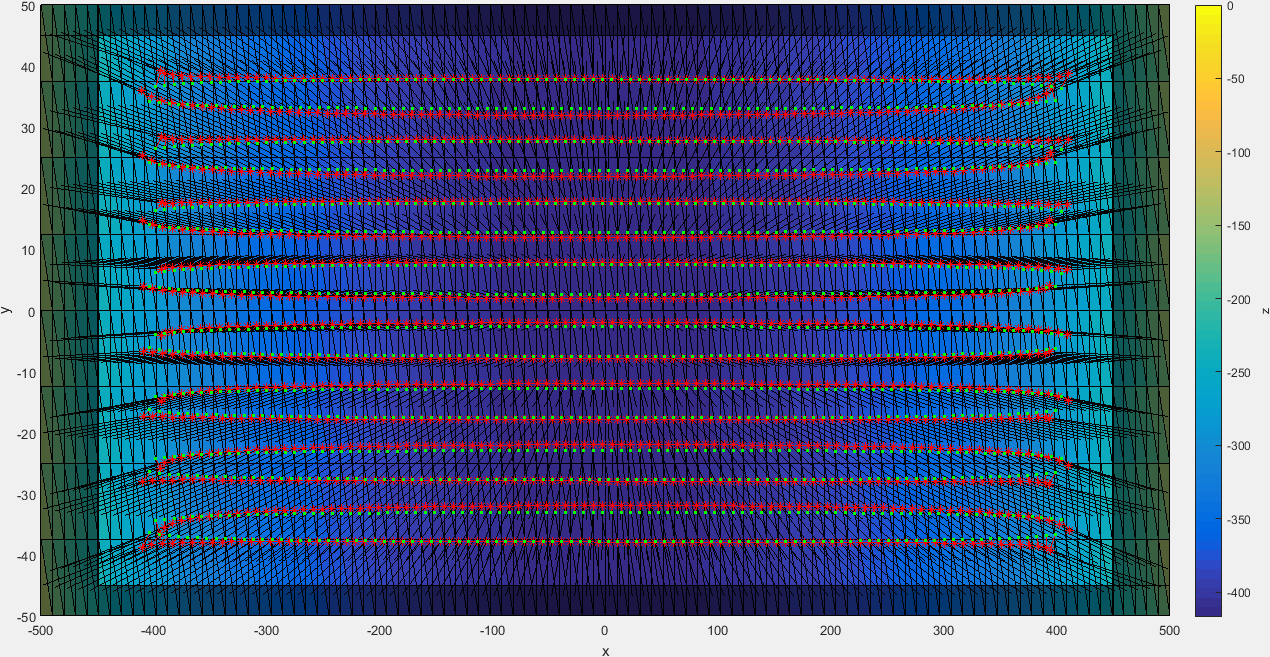
\includegraphics[width=\textwidth]{contsurf_rectangular_normal_incident_planeofsolarcell.png}
\caption{shows the average distance to the designpoint \label{contsurf_rectangular_normal_incident_planeofsolarcell}}
\end{subfigure}
\caption{continuopus surface, rectangular solar cell, optimised for normal incidence}
\end{figure}


\begin{figure}[h]
\centering
\begin{subfigure}{\textwidth}
\centering
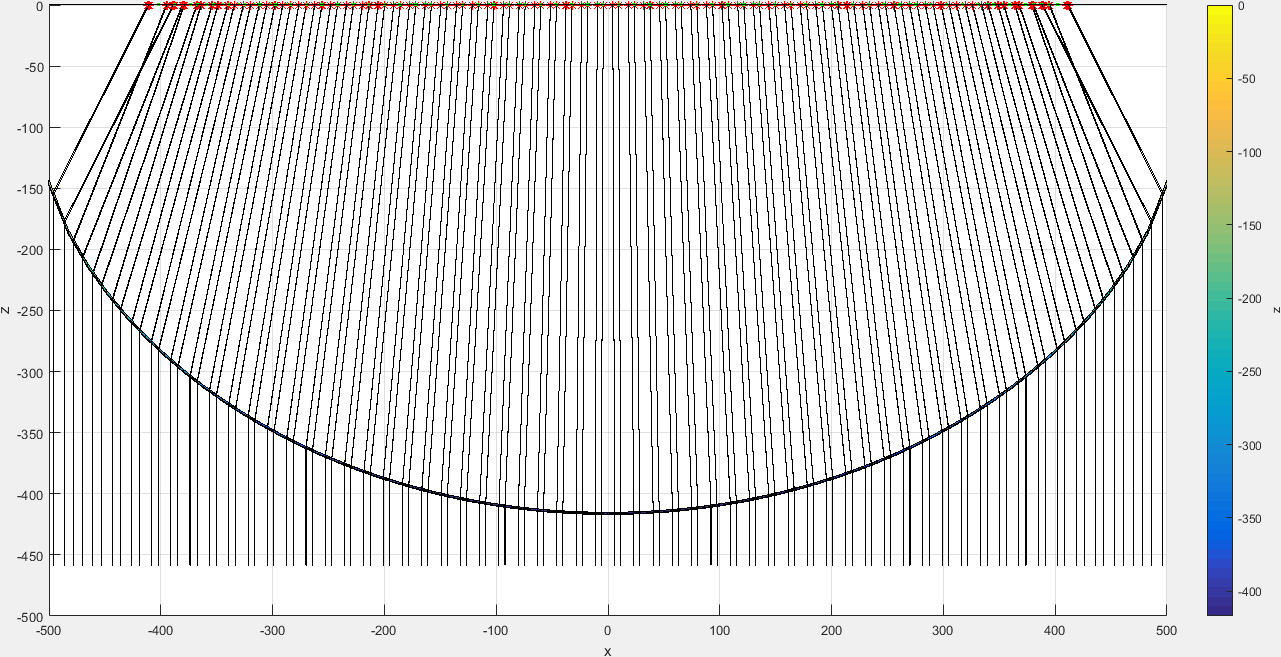
\includegraphics[width=0.48\textwidth]{contsurf_rectangular_normal_incident_view00}
\caption{\label{contsurf_rectangular_normal_incident_view00}}
\end{subfigure}
\begin{subfigure}{\textwidth}
\centering
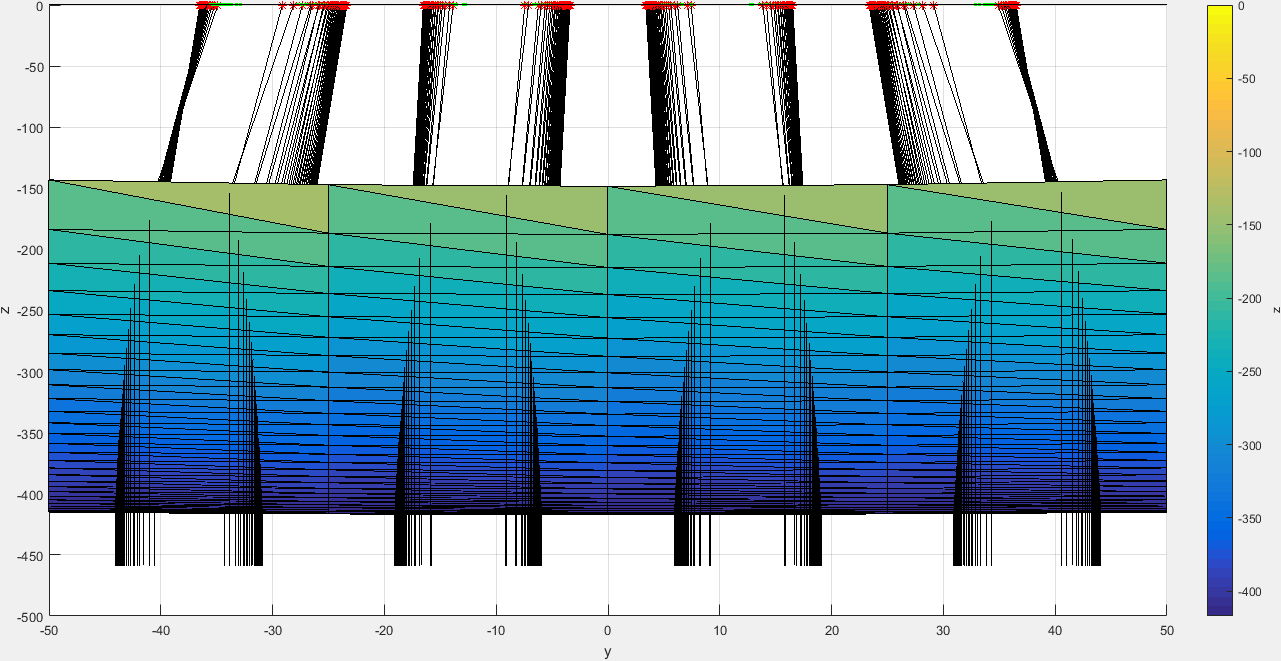
\includegraphics[width=0.48\textwidth]{contsurf_rectangular_normal_incident_view900.png}
\caption{ \label{contsurf_rectangular_normal_incident_view900}}
\end{subfigure}
\begin{subfigure}{\textwidth}
\centering
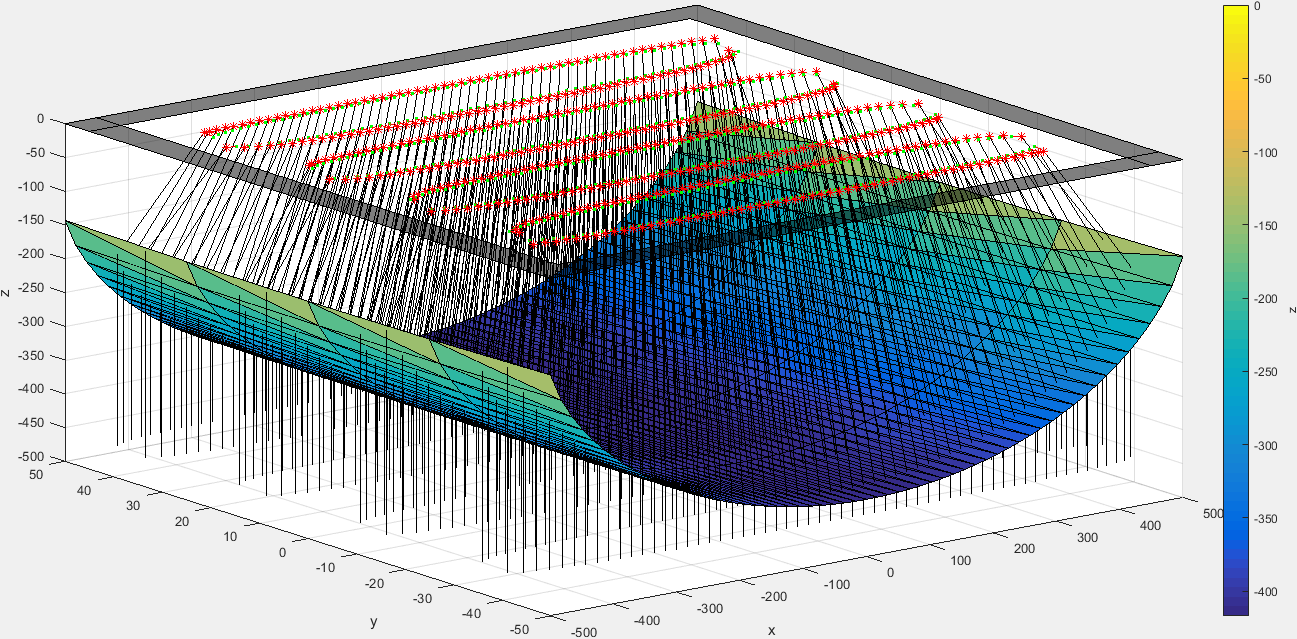
\includegraphics[width=\textwidth]{contsurf_rectangular_normal_incident_view3.png}
\caption{ \label{contsurf_rectangular_normal_incident_view3}}
\end{subfigure}
\caption{continuopus surface, rectangular solar cell, optimised for normal incidence, the solar cell is located at z=0 and the light is travelling in positive z direction}
\end{figure}


\subsection{optimised for annual improvement}

\begin{figure}[h]
\centering
\begin{subfigure}{0.45\textwidth}
\centering
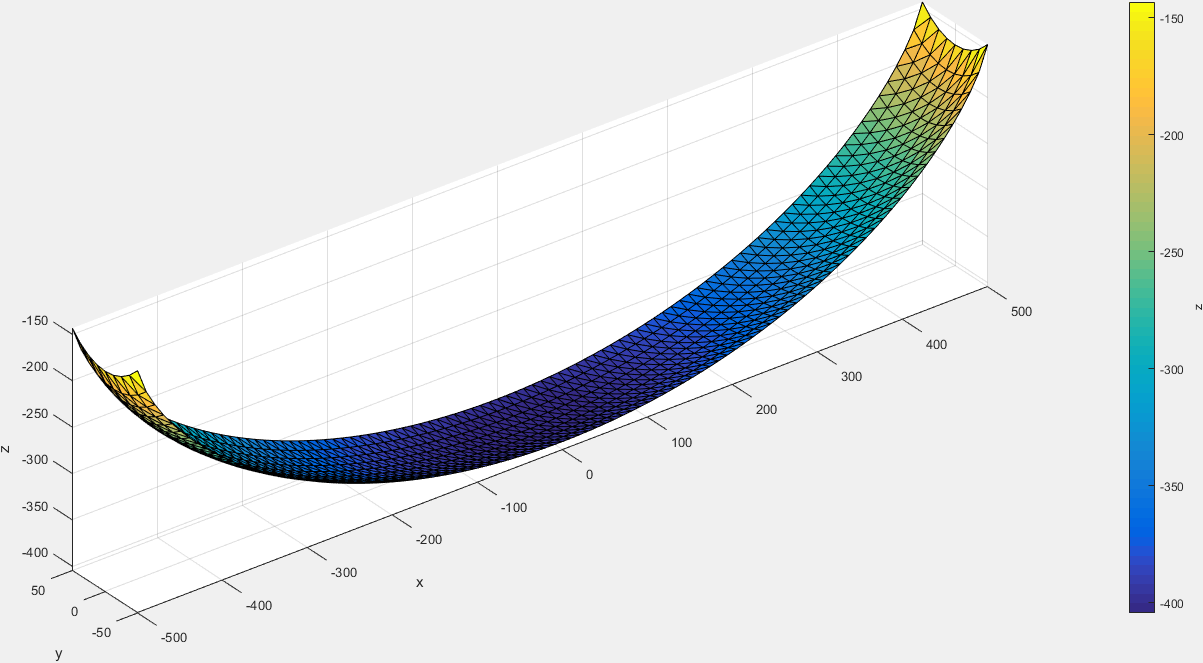
\includegraphics[width=\textwidth]{contsurf_rectangular_annualopt_surface}
\caption{the solar cell is located at z=0 and the light is travelling in positive z direction\label{contsurf_rectangular_annualopt_surface}}
\end{subfigure}
\begin{subfigure}{0.45\textwidth}
\centering
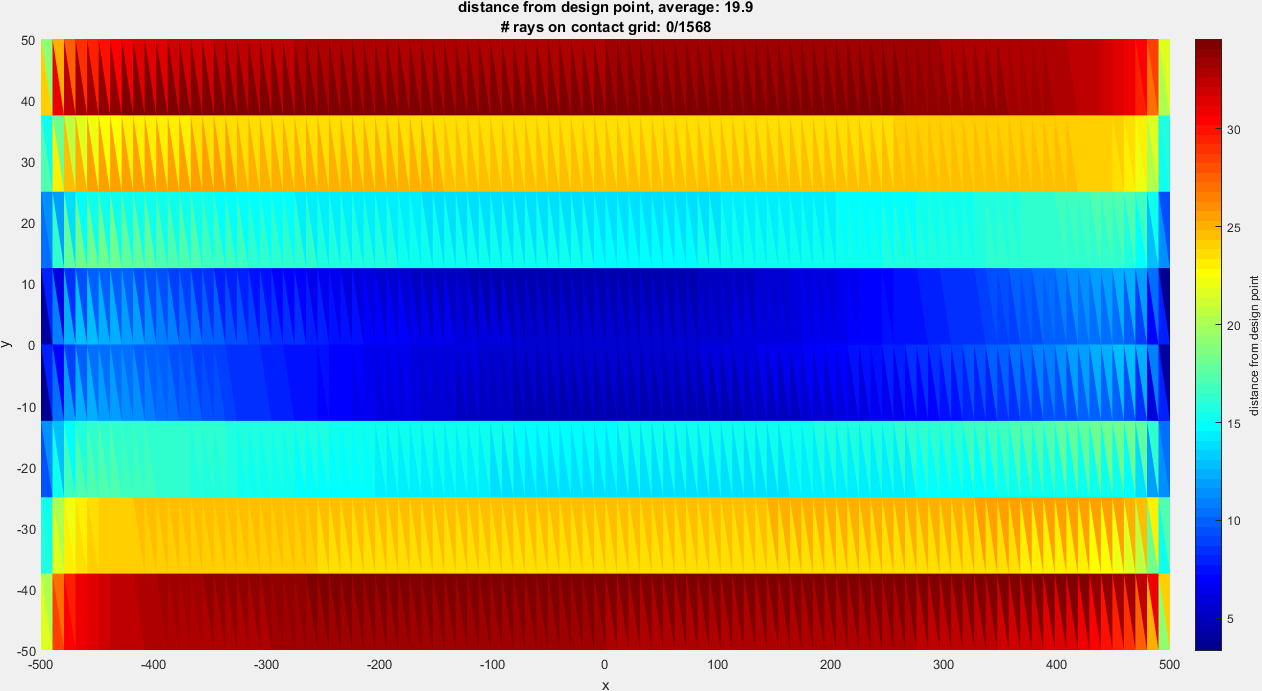
\includegraphics[width=\textwidth]{contsurf_rectangular_annualopt_average_distance.png}
\caption{shows the average distance to the designpoint \label{contsurf_rectangular_annualopt_average_distance}}
\end{subfigure}
\caption{continuopus surface, rectangular solar cell, optimised for annual improvement}
\end{figure}

\section{Simulation squared unit cell}
